\chapter{Open Questions and Further Research}\label{ch:closing}

\vspace*{-50pt}

\begin{figure}[ht]
        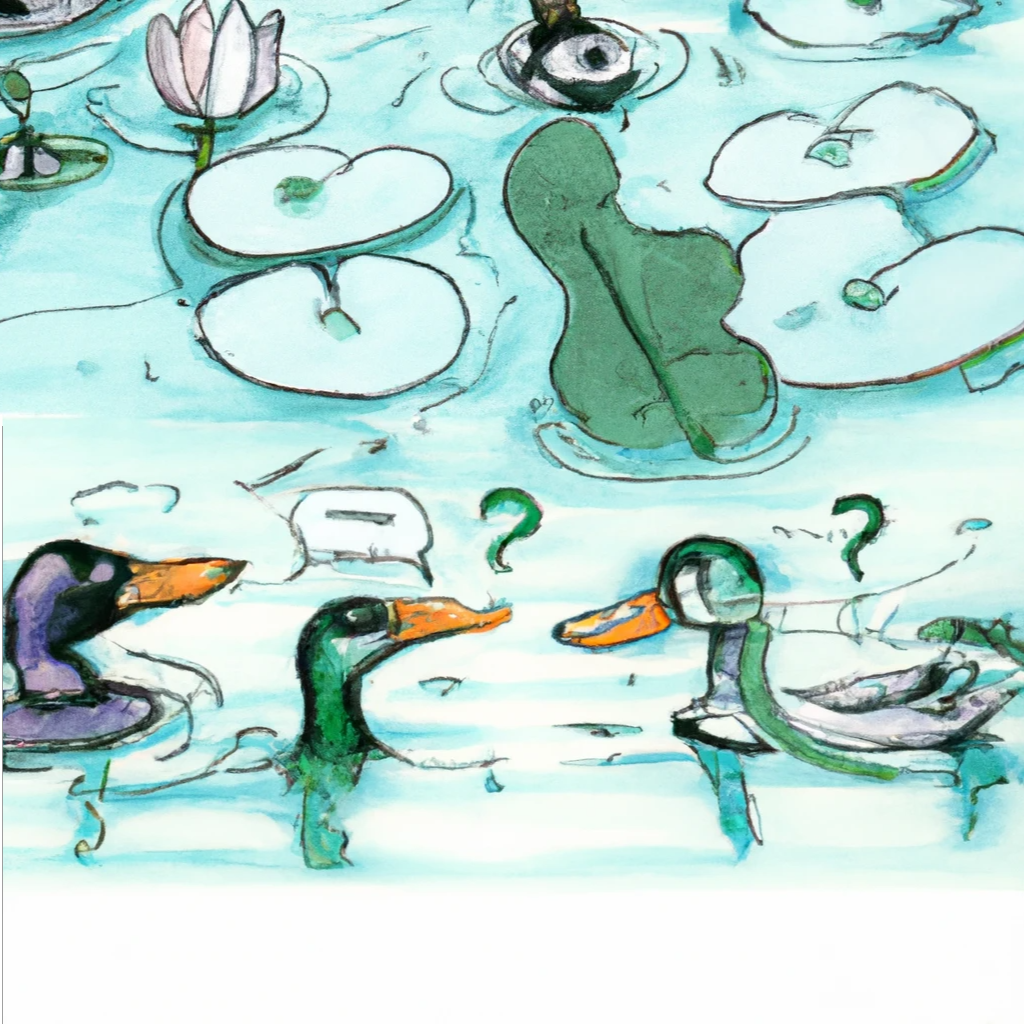
\includegraphics[width=0.35\textwidth, right]{img/further-questions.png}
        \captionsetup{textformat=empty,labelformat=blank}
        \caption[Generated with Dalle-E. Knowledge Cutoff 09-2022]{Generated with Dall-E. \url{https://labs.openai.com/}. ``more ducks asking further questions and research topics''}
\end{figure}

\epigraph{\itshape ``Peter does what he usually does when he doesn’t know what to do next: he gives up.''}{Qualityland, \textit{Marc-Uwe Kling}}

After occupying the water lilies for a couple of days, the \textit{geesiosi}s finally gave up and your ducks have the sea again for their own!
Somehow, the \sdom problem has aroused the duck's full curiosity and they start to think about the problem themselves! 
After you have shown them a polynomial kernel of size $\kernelsize \cdot k$ and that this does probably not exist for \textit{split graphs}, \textit{chordal graphs} and \textit{bipartite} graphs, they started to gather their own questions.
This is, what they have come up with:

\noindent \textbf{Improving Kernel~}
The constant of the kernel size $\kernelsize \cdot k$ is very high and the theoretical bounds are too large for practical applications. 
It would be interesting to improve them.
One idea would be the following:

\cref{rgl:rtwo} uses the fact that $N(v,w)$ can be dominated by at most four vertices: $v$,$w$ and two neighbors as a witness.
Observe that if $d(v,w) \leq 3$, this witness might be shared in an sds, because choosing one single witness on the path from $v$ to $w$ is sufficient to semitotally dominate $N(v,w)$.
Therefore $\Dvw$, $\Dv$ and $\Dw$ could be redefined to contain sets of size at most two (instead of three) which will improve the reduction. 
Note that in our analysis, the poles of a region $R$ in the \dreg $\mathfrak{R}$ satisfy $d(v,w) \leq 3$ by definition.
therefore, requiring $d(v,w) \leq 3$ would be ok and we can still assume that \cref{rgl:rtwo} has been applied for any $R \in \mathfrak{R}$.
$d(v,w)$ can be calculated in linear time and would not blow up our runtime.

\noindent \textbf{Experimental Results~}
Our analysis and its large constants refer to the worst-case scenario which tells us little about the performance applied to real-world instances.
Already Alber et al. \cite{Alber2004} noticed that this kind of reduction behaves very well in nature and showed in an experimental setting for \pdom that more than $79\%$ of the vertices and $88\%$ of the edges have been removed by their reduction rules from a sample set of random planar graphs with up to $4000$ vertices. 

\noindent \textbf{Other Open Prolems~}
The classical complexities for \textit{dually chordal} and \textit{tolerance} graphs have already been asked for by Galby et al. \cite{Galby2020} and are still open.

Furthermore, it would be interesting to complement the parameterized complexities on the hard classes we have started in this work.
open are those for \textit{circle}, \textit{chordal bipartite} and \textit{undirected path} graphs.
We think that \sdoms on \textit{chordal bipartite} graphs is at least \WONEhs-hard when parameterized by solution size, but we have been unable to prove it.
Furthermore, the reduction for \textit{circle} graphs \cite{Kloks2021} to show \NP-completeness depends on the input size, but \doms and \tdoms have already been shown to be \WONEhs-hard on \textit{circle} graphs \cite{Bousquet2012}. 
Maybe these reductions can be adjusted to show \WONEhs-hardness for \sdoms as well.
Last but not least, there exists an fpt algorithm for \doms on \textit{undirected path} graphs \cite{Figueiredo2022}. 
Does it transfer to \sdoms as well?

